\documentclass{mimosis} % Copyright (c) 2018 Bastian Rieck (MIT)
\usepackage[numbers]{natbib}
\usepackage{minted}
\usepackage{metalogo}
\usepackage{graphicx}

%%%%%%%%%%%%%%%%%%%%%%%%%%%%%%%%%%%%%%%%%%%%%%%%%%%%%%%%%%%%%%%%%%%%%%%%
% Some of my favourite personal adjustments
%
% These are the adjustments that I consider necessary for typesetting
% a nice thesis. However, they are *not* included in the template, as
% I do not want to force you to use them.

% This ensures that I am able to typeset bold font in table while still aligning the numbers
% correctly.
\usepackage{etoolbox}

\usepackage[binary-units=true]{siunitx}
\DeclareSIUnit\px{px}

\sisetup{%
  detect-all           = true,
  detect-family        = true,
  detect-mode          = true,
  detect-shape         = true,
  detect-weight        = true,
  detect-inline-weight = math,
}

%%%%%%%%%%%%%%%%%%%%%%%%%%%%%%%%%%%%%%%%%%%%%%%%%%%%%%%%%%%%%%%%%%%%%%%%
% Hyperlinks & bookmarks
%%%%%%%%%%%%%%%%%%%%%%%%%%%%%%%%%%%%%%%%%%%%%%%%%%%%%%%%%%%%%%%%%%%%%%%%

\usepackage[%
  colorlinks = true,
  citecolor  = RoyalBlue,
  linkcolor  = RoyalBlue,
  urlcolor   = RoyalBlue,
  ]{hyperref}

\usepackage{bookmark}

%%%%%%%%%%%%%%%%%%%%%%%%%%%%%%%%%%%%%%%%%%%%%%%%%%%%%%%%%%%%%%%%%%%%%%%%
% Bibliography
%%%%%%%%%%%%%%%%%%%%%%%%%%%%%%%%%%%%%%%%%%%%%%%%%%%%%%%%%%%%%%%%%%%%%%%%
%
% I like the bibliography to be extremely plain, showing only a numeric
% identifier and citing everything in simple brackets. The first names,
% if present, will be initialized. DOIs and URLs will be preserved.

% \usepackage[z
%   autocite     = plain,
%   backend      = bibtex,
%   doi          = true,
%   url          = true,
%   giveninits   = true,
%   hyperref     = true,
%   maxbibnames  = 99,
%   maxcitenames = 99,
%   sortcites    = true,
%   style        = numeric,
%   ]{biblatex}

%\input{bibliography-mimosis}
%\bibliography{Thesis}

%%%%%%%%%%%%%%%%%%%%%%%%%%%%%%%%%%%%%%%%%%%%%%%%%%%%%%%%%%%%%%%%%%%%%%%%
% Fonts
%%%%%%%%%%%%%%%%%%%%%%%%%%%%%%%%%%%%%%%%%%%%%%%%%%%%%%%%%%%%%%%%%%%%%%%%

\ifxetexorluatex
  \setmainfont{Minion Pro}
\else
  \usepackage[lf]{ebgaramond}
  \usepackage[oldstyle,scale=0.7]{sourcecodepro}
  \singlespacing
\fi

\renewcommand{\th}{\textsuperscript{\textup{th}}\xspace}

\newacronym[description={Principal component analysis}]{PCA}{PCA}{principal component analysis}
\newacronym                                            {SNF}{SNF}{Smith normal form}
\newacronym[description={Topological data analysis}]   {TDA}{TDA}{topological data analysis}

\newglossaryentry{LaTeX}{%
  name        = {\LaTeX},
  description = {A document preparation system},
  sort        = {LaTeX},
}

\newglossaryentry{Real numbers}{%
  name        = {$\real$},
  description = {The set of real numbers},
  sort        = {Real numbers},
}

\makeindex
\makeglossaries

%%%%%%%%%%%%%%%%%%%%%%%%%%%%%%%%%%%%%%%%%%%%%%%%%%%%%%%%%%%%%%%%%%%%%%%%
% Incipit
%%%%%%%%%%%%%%%%%%%%%%%%%%%%%%%%%%%%%%%%%%%%%%%%%%%%%%%%%%%%%%%%%%%%%%%%

\title{\texttt{A Blockchain Enabled WS Agreements Framework}} %Autonomous Negotiation of Tamper Proof Webservice Agreements.
\subtitle{Research Proposal}
\author{Stefan Starflinger}

\begin{document}

\frontmatter
  \begin{titlepage}
  \vspace*{5cm}
  \makeatletter
  \begin{center}
    \begin{Huge}
      \@title
    \end{Huge}\\[0.1cm]
    %
    \begin{Large}
      \@subtitle
    \end{Large}\\
    %
    \emph{by}\\
    \@author
    %
    \vfill
    A document submitted in partial fulfillment
    of the requirements for the degree of\\
    \emph{Master of Science}\\
    at\\
    \textsc{University of Vienna}\\
    \vspace{0.5cm}
    \includegraphics*[width=80px]{logo.png}
  \end{center}
  \makeatother
\end{titlepage}

\newpage
\null
\thispagestyle{empty}
\newpage

  \begin{center}
  \textsc{Abstract}
\end{center}
%
\noindent
%
Scientific documents often use \LaTeX{} for typesetting. While numerous
packages and templates exist, it makes sense to create a new one. Just
because.


  \tableofcontents

\mainmatter

  %%%%%%%%%%%%%%%%%%%%%%%%%%%%%%%%%%%%%%%%%%%%%%%%%%%%%%%%%%%%%%%%%%%%%%%%
\chapter{Introduction}
%%%%%%%%%%%%%%%%%%%%%%%%%%%%%%%%%%%%%%%%%%%%%%%%%%%%%%%%%%%%%%%%%%%%%%%%

\begin{center}
  \begin{minipage}{0.5\textwidth}
    \begin{small}
      In which the reasons for creating this package are laid bare for the
      whole world to see and we encounter some usage guidelines.
    \end{small}
  \end{minipage}
  \vspace{0.5cm}
\end{center}

\noindent This package contains a minimal, modern template for writing your
thesis. While originally meant to be used for a Ph.\,D.\ thesis, you can
equally well use it for your honour thesis, bachelor thesis, and so
on---some adjustments may be necessary, though.

%%%%%%%%%%%%%%%%%%%%%%%%%%%%%%%%%%%%%%%%%%%%%%%%%%%%%%%%%%%%%%%%%%%%%%%%
\section{Why?}
%%%%%%%%%%%%%%%%%%%%%%%%%%%%%%%%%%%%%%%%%%%%%%%%%%%%%%%%%%%%%%%%%%%%%%%%

I was not satisfied with the available templates for \LaTeX{} and wanted
to heed the style advice given by people such as Robert
Bringhurst~\cite{Bringhurst12} or Edward R.\
Tufte~\cite{Tufte90,Tufte01}. While there \emph{are} some packages out
there that attempt to emulate these styles, I found them to be either
too bloated, too playful, or too constraining. This template attempts to
produce a beautiful look without having to resort to any sort of hacks.
I hope you like it.

%%%%%%%%%%%%%%%%%%%%%%%%%%%%%%%%%%%%%%%%%%%%%%%%%%%%%%%%%%%%%%%%%%%%%%%%
\section{How?}
%%%%%%%%%%%%%%%%%%%%%%%%%%%%%%%%%%%%%%%%%%%%%%%%%%%%%%%%%%%%%%%%%%%%%%%%

The package tries to be easy to use. If you are satisfied with the
default settings, just add
%
\begin{verbatim}
\documentclass{mimosis}
\end{verbatim}
%
at the beginning of your document. This is sufficient to use the class.
It is possible to build your document using either \LaTeX|, \XeLaTeX, or
\LuaLaTeX. I personally prefer one of the latter two because they make
it easier to select proper fonts.

%%%%%%%%%%%%%%%%%%%%%%%%%%%%%%%%%%%%%%%%%%%%%%%%%%%%%%%%%%%%%%%%%%%%%%%%
\section{Features}
%%%%%%%%%%%%%%%%%%%%%%%%%%%%%%%%%%%%%%%%%%%%%%%%%%%%%%%%%%%%%%%%%%%%%%%%

%%%%%%%%%%%%%%%%%%%%%%%%%%%%%%%%%%%%%%%%%%%%%%%%%%%%%%%%%%%%%%%%%%%%%%%%
\begin{table}
  \centering
  \begin{tabular}{ll}
    \toprule
    \textbf{Package}      & \textbf{Purpose}\\
    \midrule
      \texttt{amsmath}          & Basic mathematical typography\\
      \texttt{amsthm}           & Basic mathematical environments for proofs etc.\\
      \texttt{booktabs}         & Typographically light rules for tables\\
      \texttt{bookmarks}        & Bookmarks in the resulting PDF\\
      \texttt{dsfont}           & Double-stroke font for mathematical concepts\\
      \texttt{graphicx}         & Graphics\\
      \texttt{hyperref}         & Hyperlinks\\
      \texttt{multirow}         & Permits table content to span multiple rows or columns\\ 
      \texttt{paralist}         & Paragraph~(`in-line') lists and compact enumerations\\
      \texttt{scrlayer-scrpage} & Page headings\\
      \texttt{setspace}         & Line spacing\\
      \texttt{siunitx}          & Proper typesetting of units\\
      \texttt{subcaption} & Proper sub-captions for figures\\
    \bottomrule
  \end{tabular}
  \caption{%
    A list of the most relevant packages required~(and automatically imported) by this template.
  }
  \label{tab:Packages}
\end{table}
%%%%%%%%%%%%%%%%%%%%%%%%%%%%%%%%%%%%%%%%%%%%%%%%%%%%%%%%%%%%%%%%%%%%%%%%

The template automatically imports numerous convenience packages that
aid in your typesetting process. \autoref{tab:Packages} lists the
most important ones. Let's briefly discuss some examples below. Please
refer to the source code for more demonstrations.

%%%%%%%%%%%%%%%%%%%%%%%%%%%%%%%%%%%%%%%%%%%%%%%%%%%%%%%%%%%%%%%%%%%%%%%%
\subsection{Typesetting mathematics}
%%%%%%%%%%%%%%%%%%%%%%%%%%%%%%%%%%%%%%%%%%%%%%%%%%%%%%%%%%%%%%%%%%%%%%%%

This template uses \verb|amsmath| and \verb|amssymb|, which are the
de-facto standard for typesetting mathematics. Use numbered equations
using the \verb|equation| environment.
%
If you want to show multiple equations and align them, use the
\verb|align| environment:
%
\begin{align}
    V &:= \{ 1, 2, \dots \}\\
    E &:= \big\{ \left(u,v\right) \mid \dist\left(p_u, p_v\right) \leq \epsilon \big\}
\end{align}
%
Define new mathematical operators using \verb|\DeclareMathOperator|.
Some operators are already pre-defined by the template, such as the
distance between two objects. Please see the template for some examples. 
%
Moreover, this template contains a correct differential operator. Use \verb|\diff| to typeset the differential of integrals:
%
\begin{equation}
  f(u) := \int_{v \in \domain}\dist(u,v)\diff{v}
\end{equation}
%
You can see that, as a courtesy towards most mathematicians, this
template gives you the possibility to refer to the real numbers~$\real$
and the domain~$\domain$ of some function. Take a look at the source for
more examples. By the way, the template comes with spacing fixes for the
automated placement of brackets.

%%%%%%%%%%%%%%%%%%%%%%%%%%%%%%%%%%%%%%%%%%%%%%%%%%%%%%%%%%%%%%%%%%%%%%%%
\subsection{Typesetting text}
%%%%%%%%%%%%%%%%%%%%%%%%%%%%%%%%%%%%%%%%%%%%%%%%%%%%%%%%%%%%%%%%%%%%%%%%

Along with the standard environments, this template offers
\verb|paralist| for lists within paragraphs.
%
Here's a quick example: The American constitution speaks, among others, of
%
\begin{inparaenum}[(i)]
  \item life
  \item liberty
  \item the pursuit of happiness.
\end{inparaenum}
%
These should be added in equal measure to your own conduct. To typeset
units correctly, use the \verb|siunitx| package. For example, you might
want to restrict your daily intake of liberty to \SI{750}{\milli\gram}.

Likewise, as a small pet peeve of mine, I offer specific operators for \emph{ordinals}. Use \verb|\th| to typeset things like July~4\th correctly. Or, if you are referring to the 2\nd edition of a book, please use \verb|\nd|. Likewise, if you came in 3\rd in a marathon, use \verb|\rd|. This is my 1\st rule.

%%%%%%%%%%%%%%%%%%%%%%%%%%%%%%%%%%%%%%%%%%%%%%%%%%%%%%%%%%%%%%%%%%%%%%%%
\section{Changing things}
%%%%%%%%%%%%%%%%%%%%%%%%%%%%%%%%%%%%%%%%%%%%%%%%%%%%%%%%%%%%%%%%%%%%%%%%

Since this class heavily relies on the \verb|scrbook| class, you can use
\emph{their} styling commands in order to change the look of things. For
example, if you want to change the text in sections to \textbf{bold} you
can just use
%
\begin{verbatim}
  \setkomafont{sectioning}{\normalfont\bfseries}
\end{verbatim}
%
at the end of the document preamble---you don't have to modify the class
file for this. Please consult the source code for more information.

  % !TEX root = ../Thesis.tex
%%%%%%%%%%%%%%%%%%%%%%%%%%%%%%%%%%%%%%%%%%%%%%%%%%%%%%%%%%%%%%%%%%%%%%%%
\chapter{Blockchain}
%%%%%%%%%%%%%%%%%%%%%%%%%%%%%%%%%%%%%%%%%%%%%%%%%%%%%%%%%%%%%%%%%%%%%%%%

Blockchain technology was developed in the wake of the 2008 financial crisis. Today, it could help shape the future of a borderless financial world. It eradicates the need for a trusted third party, instead we lay our trust in a public protocol. The blockchain protocol combines a reward system with a consensus algorithm in a novel way, which keeps the system secure and stable. As an example, a bad actor would earn more money if he helped secure the system than if he tried to attack it.

The reason trust is no longer necessary is that all of the code is open source. Thus, the protocol is easily available. This means, given enough time, anyone can understand the protocol and validate that it is does what it advertises. In the case of Bitcoin, an example of such a guarantee would be that only the holder of the private key, of a unspent transaction output (UTXO) can sign a transaction for his Bitcoin address. There are currently many different implementations of the Blockchain technology and that is partly because it is difficult to find a protocol that we can all agree upon.

% Further elaborate these thoughts
Transactions by the ledger are pseudonymous. This means that future revelations of identity can be disastrous. It is the modern way of storing money under the bed. Well, not quite the Blockchain has many usecases although most have yet to be realized; one thing is sure, it is not solely a currency revolution.

How might the Blockchain technology be relevant in trying to reach an agreement between a provider and a consumer. When you face this decision, the first question should be:
\begin{verbatim}
Do you trust your negotiation partner? 
\end{verbatim}
If the answer is \emph{yes}, then it is not necessary for you to use a Blockchain. Yet if the answer is \emph{maybe} or \emph{no} then a Blockchain might be a good idea. Below we will look at what kind of Blockchain might be suitable for bilateral negotiation and how the individuals would benefit from using a Blockchain instead of a regular database.


%TODO write what aspects we are looking for
%%%%%%%%%%%%%%%%%%%%%%%%%%%%%%%%%%%%%%%%%%%%%%%%%%%%%%%%%%%%%%%%%%%%%%%%
\subsection{Bitcoin}
%%%%%%%%%%%%%%%%%%%%%%%%%%%%%%%%%%%%%%%%%%%%%%%%%%%%%%%%%%%%%%%%%%%%%%%%

The idea for a peer to peer cash system named Bitcoin was first brought forward by Satoshi Nakamoto in his paper \cite{nakamoto2008bitcoin}. There he described a electronic cash system that does not need a trusted third party to perform payments. Together with a group of developers Satoshi Nakamoto went on a mission, to bring his idea to life. He drew his motivation from the 2008 financial crisis, where banks brought ruin over the global financial markets. The fundamental idea behind Bitcoin is now known as the Blockchain, which has the potential to revolutionize our industry.

%%%%%%%%%%%%%%%%%%%%%%%%%%%%%%%%%%%%%%%%%%%%%%%%%%%%%%%%%%%%%%%%%%%%%%%%
\subsubsection{Double Spending}

The major crux, of realizing an electronic cash system, is the double spending problem. Basically, it sums up to ensuring that when Alice receives a payment from Bob, how can she be sure that Bob has not already spent that money somewhere else. That is where the distributed ledger technology (DLT) comes into play. It is a basic ledger equipped with cryptographic proofs. To prevent double spending, the ledger is secured through a mechanism called proof of work.

\subsubsection{Proof of Work} 

The cornerstone of why Bitcoin works, is its Proof of Work (PoW) algorithm. It rewards honest nodes in the peer to peer network and punishes dishonest nodes, at the same time. The nodes that secure the network (the honest nodes) have the possibility to receive a reward for their work. The work that needs to be done serves only to reach consensus and keep the network secure. Honest nodes that secure the network are also known as miners. These miners perform hash operations and the first miner to calculate a hash lower than the difficulty is rewarded by the protocol with a predetermined amount of Bitcoin. Further, the algorithm used for mining is the hashcash  $ sha256^2 $. %\cite{TODO}.  

As an analogy one can image the protocol to work similar to the following. Imagine the Blockchain as a puzzle, where each piece only has two sides. This would mean that a new piece can only be placed at the end of the current chain. The image depicted by each puzzle piece are the transactions in a block. The miners, as quickly as possible, take out pieces from a huge bag. To be more precise, in the bag that the miners choose puzzle pieces from, there are around $2^{256} = 1.158 * 10^{77}$ possible combinations. Only a small subset of the combinations determined by the difficulty, is eligible for a reward. They check if the piece fits, if it does they pass a copy of that puzzle piece to all other nodes and get a reward from the protocol. Although, the other miners only accept the piece if the image fits to the previous pieces i.e. if the transactions in the block are not already spent.

%%%%%%%%%%%%%%%%%%%%%%%%%%%%%%%%%%%%%%%%%%%%%%%%%%%%%%%%%%%%%%%%%%%%%%%%
\subsection{Ethereum}
%%%%%%%%%%%%%%%%%%%%%%%%%%%%%%%%%%%%%%%%%%%%%%%%%%%%%%%%%%%%%%%%%%%%%%%%
First proposed by Vitalik Buterin in 2013 as an alternative to the Bitcoin. The general idea was to create a turing-complete language that can be run on the Blockchain. This idea was novel compared to the simple scripting language that Bitcoin implements. Through the turing complete language Buterin gave developers a playground on which they could develop their trust-less decentralized ideas. These are currently called decentralized applications or dapps short. 

Previously called the DAO project. It allows users to build decentralized applications (dapps) on top of its Blockchain. It has a quite different technical implementation than Bitcoin but follows the Blockchain fundamentals. From all of the current projects Ethereum is one of the most promising. 

Ethereum is built with merkle trees.

Ethereum allows users to write smart contracts using its solidity programming language. The programming language is compiled down and run on a virtual machine similar to what Javascript does. This VM is called the Ethereum Virtual Machine (EVM). 

%Proof of work

%merkle tree

%%%%%%%%%%%%%%%%%%%%%%%%%%%%%%%%%%%%%%%%%%%%%%%%%%%%%%%%%%%%%%%%%%%%%%%%
\subsection{Iota}
%%%%%%%%%%%%%%%%%%%%%%%%%%%%%%%%%%%%%%%%%%%%%%%%%%%%%%%%%%%%%%%%%%%%%%%%
Bitcoin being the first implementation of a distributed ledger has quite some flaws. Iota tries to tackle these flaws, keeping the internet of things (IOT) in mind. For example, with the Bitcoin protocol micro transactions are not economically viable, since the transaction fee is too high. In the whitepaper \cite{iota_wp} problems with the Bitcoin protocol are discussed by presenting an alternative solution, Iota.

One of the key points with the Iota distributed ledger is that it does not have transaction fees. Instead, before broadcasting a transaction, peers need to secure the network by performing a proof of work for two previous transactions. In doing so, Iota does not split the network in two groups, the miners and the users. Another key is that instead of having a single chain Iota went for a graph approach, a Directed Acyclic Graph (DAG) to be precise.
%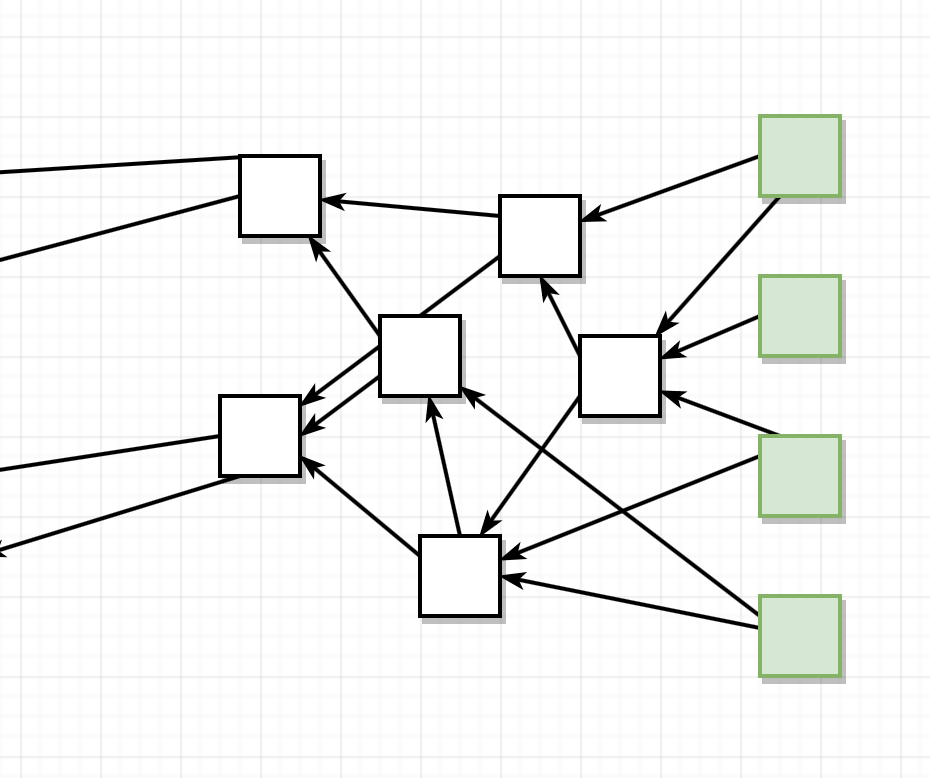
\includegraphics{tangle.png}
%%%%%%%%%%%%%%%%%%%%%%%%%%%%%%%%%%%%%%%%%%%%%%%%%%%%%%%%%%%%%%%%%%%%%%%%
\subsection{Stellar}
%%%%%%%%%%%%%%%%%%%%%%%%%%%%%%%%%%%%%%%%%%%%%%%%%%%%%%%%%%%%%%%%%%%%%%%%

%%%%%%%%%%%%%%%%%%%%%%%%%%%%%%%%%%%%%%%%%%%%%%%%%%%%%%%%%%%%%%%%%%%%%%%%
\subsection{Cardano}
%%%%%%%%%%%%%%%%%%%%%%%%%%%%%%%%%%%%%%%%%%%%%%%%%%%%%%%%%%%%%%%%%%%%%%%%

%%%%%%%%%%%%%%%%%%%%%%%%%%%%%%%%%%%%%%%%%%%%%%%%%%%%%%%%%%%%%%%%%%%%%%%%
\subsection{Neo}
%%%%%%%%%%%%%%%%%%%%%%%%%%%%%%%%%%%%%%%%%%%%%%%%%%%%%%%%%%%%%%%%%%%%%%%%
Similar to Ethereum being developed in China

%%%%%%%%%%%%%%%%%%%%%%%%%%%%%%%%%%%%%%%%%%%%%%%%%%%%%%%%%%%%%%%%%%%%%%%%
\subsection{Hyperledger}
%%%%%%%%%%%%%%%%%%%%%%%%%%%%%%%%%%%%%%%%%%%%%%%%%%%%%%%%%%%%%%%%%%%%%%%%
A private implementation of Ethereum with a pluggable consensus algorithm. Open sourced by the linux foundation.

%%%%%%%%%%%%%%%%%%%%%%%%%%%%%%%%%%%%%%%%%%%%%%%%%%%%%%%%%%%%%%%%%%%%%%%%
\section{Comparing Implementations}
%%%%%%%%%%%%%%%%%%%%%%%%%%%%%%%%%%%%%%%%%%%%%%%%%%%%%%%%%%%%%%%%%%%%%%%%
In the following sections we will look more closely at different implementations of the Blockchain technology. As of this writing there are more than a thousand cryptocurrencies. To get a good overview we will look at different approaches and exclude hardforks/clones, ICOs and cryptocurrencies without a working product.

%%%%%%%%%%%%%%%%%%%%%%%%%%%%%%%%%%%%%%%%%%%%%%%%%%%%%%%%%%%%%%%%%%%%%%%%
\begin{table}
  %\centering
  \begin{tabular}{llllll}
    \toprule
    \textbf{Blockchain} & \textbf{Genesis} & \textbf{Consensus} & \textbf{\# Clients} & \textbf{Replications} & \textbf{Mining/Security} \\
    \midrule
      \texttt{Bitcoin} & 2009 & Proof of Work & 1 & 1234 \\
      \texttt{Ethereum} & 2009 & Proof of Work & 1 & 1234 \\
      \texttt{Iota} & 2009 & Proof of Work & 1 & 1234 \\
      \texttt{Stellar} & 2009 & Proof of Work & 1 & 1234 \\
      \texttt{Cardano} & 2009 & Proof of Work & 1 & 1234 \\
      \texttt{Neo} & 2009 & Proof of Work & 1 & 1234 \\
      \texttt{Hyperledger} & 2009 & Proof of Work & 1 & 1234 \\
    \bottomrule
  \end{tabular}
  \caption{%
    A table comparing different distributed ledger technologies.
  }
  \label{tab:Packages}
\end{table}
%%%%%%%%%%%%%%%%%%%%%%%%%%%%%%%%%%%%%%%%%%%%%%%%%%%%%%%%%%%%%%%%%%%%%%%%


%%%%%%%%%%%%%%%%%%%%%%%%%%%%%%%%%%%%%%%%%%%%%%%%%%%%%%%%%%%%%%%%%%%%%%%%
\section{Choosing an Implementation}
%%%%%%%%%%%%%%%%%%%%%%%%%%%%%%%%%%%%%%%%%%%%%%%%%%%%%%%%%%%%%%%%%%%%%%%%



  %%%%%%%%%%%%%%%%%%%%%%%%%%%%%%%%%%%%%%%%%%%%%%%%%%%%%%%%%%%%%%%%%%%%%%%%
\chapter{Web Service Agreements}
%%%%%%%%%%%%%%%%%%%%%%%%%%%%%%%%%%%%%%%%%%%%%%%%%%%%%%%%%%%%%%%%%%%%%%%%

\begin{center}
  \begin{minipage}{0.5\textwidth}
    \begin{small}
      Establishing agreements typically between a provider and a consumer~\cite{andrieux2007web}.
    \end{small}
  \end{minipage}
  \vspace{0.5cm}
\end{center}

In this chapter we will look into more detail about how a provider and a consumer can come to an agreement, what information needs to be exchanged and what kind of interface is necessary to store the relevant information in the blockchain.[]

%%%%%%%%%%%%%%%%%%%%%%%%%%%%%%%%%%%%%%%%%%%%%%%%%%%%%%%%%%%%%%%%%%%%%%%%
\section{Service Level Agreements (SLA)}
%%%%%%%%%%%%%%%%%%%%%%%%%%%%%%%%%%%%%%%%%%%%%%%%%%%%%%%%%%%%%%%%%%%%%%%%
Service level agreements are legally binding agreements about the service that is provided to a consumer. Similarly Irfan UI Haq defined it as, "A Service Level Agreement is a formal, legal contract between a service provider and a consumer that specifies, in quantifiable terms, what service level guarantees the service provider will deliver, and it defines the consequences (penalties) if the service provider fails to follow through with said commitments." \cite{TODO PHD THESISIRFAN}. To this definition there are two main parts. The first, is the commitment that there must be a definition of the commitment that the provider is willing to offer the consumer. The second, is the punishment that is due if the provider is not able to uphold his commitment. Before a SLA is binding it needs to go through a negotiation process, which will be looked at more closely in a later chapter. For now, it is enough to realize that it is an agreement between two parties over a range of attributes that a service must provide.

%%%%%%%%%%%%%%%%%%%%%%%%%%%%%%%%%%%%%%%%%%%%%%%%%%%%%%%%%%%%%%%%%%%%%%%%
\section{Web Service Agreement Specification}
%%%%%%%%%%%%%%%%%%%%%%%%%%%%%%%%%%%%%%%%%%%%%%%%%%%%%%%%%%%%%%%%%%%%%%%%
This specification provides templates and a semantic description of the elements in an agreement using the XML markup language. 

%%%%%%%%%%%%%%%%%%%%%%%%%%%%%%%%%%%%%%%%%%%%%%%%%%%%%%%%%%%%%%%%%%%%%%%%
\subsection{JSON representation}
%%%%%%%%%%%%%%%%%%%%%%%%%%%%%%%%%%%%%%%%%%%%%%%%%%%%%%%%%%%%%%%%%%%%%%%%
In order to better understand the WS-Agreement Specification we wrote up a JSON representation of the example XML schema described.

The abstract overview of an Agreement would look like this:
\begin{minted}{json}
{
  "Agreement": {
    "id": "Unique identifier of the agreement version (increment identifier for each new version)",
    "Name": "Optional, name of the agreement",
    "Context": "Who is involved, what the services are and the duration.",
    "Terms": "Terms of the agreement with one or more service definition terms and zero or more guarantee terms."
  }
}
\end{minted}

Looking more closely at the Context of the Agreement.
\begin{minted}{json}
{
  "Context": {
    "AgreementInitiator": "The entity that initiates the agreement",
    "AgreementResponder": "Optional, entity that responds to the agreement creation request.",
    "ServiceProvider": "The entity that provides the service",
    "ExpirationTime": "The date-time when this agreement is no longer valid",
    "TemplateId": "Required, The Id of the template this agreement was built upon",
    "TemplateName": "Optional, The name of the template this agreement was built upon",
    "any": "Additional values may be specified",
  }
}
\end{minted}

Lastly the Agreement consists of multiple terms
\begin{minted}{json}
{
  "Terms": {
    "Service": {
      "DescriptionTerm": {
        "Name": "local name",
        "ServiceName": "global name",
        "description": "Additional values to describe the service"
      }
      "Reference": {
        "Name": "local name",
        "ServiceName": "global name",
        "reference": ""
      }
      "Properties": {
        "Name": "local name",
        "ServiceName": "global name",
        "Variables": [{
          "Name": "Gas",
          "Metric": "barrels" ,
          "Location": "reference e.g. XPATH",
        }]
      }
    },
    "Guarantee": {
      "Name": "specify promises and penalties",
      "Obligated": "",
      "ServiceScope": {
        "Name": "",
        "Value": "",
      }
      "QualifyingCondition": "",
      "ServiceLevelObjective": "",
      "BusinessValueList": ""
    }
  }
}
\end{minted}

  %%%%%%%%%%%%%%%%%%%%%%%%%%%%%%%%%%%%%%%%%%%%%%%%%%%%%%%%%%%%%%%%%%%%%%%%
\chapter{Negotiation}
%%%%%%%%%%%%%%%%%%%%%%%%%%%%%%%%%%%%%%%%%%%%%%%%%%%%%%%%%%%%%%%%%%%%%%%%

\begin{center}
  \begin{minipage}{0.5\textwidth}
    \begin{small}
      In which the reasons for creating this package are laid bare for the
      whole world to see and we encounter some usage guidelines.
    \end{small}
  \end{minipage}
  \vspace{0.5cm}
\end{center}

\noindent This package contains a minimal, modern template for writing your
thesis. While originally meant to be used for a Ph.\,D.\ thesis, you can
equally well use it for your honour thesis, bachelor thesis, and so
on---some adjustments may be necessary, though.

%%%%%%%%%%%%%%%%%%%%%%%%%%%%%%%%%%%%%%%%%%%%%%%%%%%%%%%%%%%%%%%%%%%%%%%%
\section{Why?}
%%%%%%%%%%%%%%%%%%%%%%%%%%%%%%%%%%%%%%%%%%%%%%%%%%%%%%%%%%%%%%%%%%%%%%%%

I was not satisfied with the available templates for \LaTeX{} and wanted
to heed the style advice given by people such as Robert
Bringhurst~\cite{Bringhurst12} or Edward R.\
Tufte~\cite{Tufte90,Tufte01}. While there \emph{are} some packages out
there that attempt to emulate these styles, I found them to be either
too bloated, too playful, or too constraining. This template attempts to
produce a beautiful look without having to resort to any sort of hacks.
I hope you like it.

  %%%%%%%%%%%%%%%%%%%%%%%%%%%%%%%%%%%%%%%%%%%%%%%%%%%%%%%%%%%%%%%%%%%%%%%%
\chapter{Contracts}
%%%%%%%%%%%%%%%%%%%%%%%%%%%%%%%%%%%%%%%%%%%%%%%%%%%%%%%%%%%%%%%%%%%%%%%%

\begin{center}
  \begin{minipage}{0.5\textwidth}
    \begin{small}
      In which the reasons for creating this package are laid bare for the
      whole world to see and we encounter some usage guidelines.
    \end{small}
  \end{minipage}
  \vspace{0.5cm}
\end{center}

\noindent This package contains a minimal, modern template for writing your
thesis. While originally meant to be used for a Ph.\,D.\ thesis, you can
equally well use it for your honour thesis, bachelor thesis, and so
on---some adjustments may be necessary, though.

%%%%%%%%%%%%%%%%%%%%%%%%%%%%%%%%%%%%%%%%%%%%%%%%%%%%%%%%%%%%%%%%%%%%%%%%
\section{Why?}
%%%%%%%%%%%%%%%%%%%%%%%%%%%%%%%%%%%%%%%%%%%%%%%%%%%%%%%%%%%%%%%%%%%%%%%%

I was not satisfied with the available templates for \LaTeX{} and wanted
to heed the style advice given by people such as Robert
Bringhurst~\cite{Bringhurst12} or Edward R.\
Tufte~\cite{Tufte90,Tufte01}. While there \emph{are} some packages out
there that attempt to emulate these styles, I found them to be either
too bloated, too playful, or too constraining. This template attempts to
produce a beautiful look without having to resort to any sort of hacks.
I hope you like it.

%%%%%%%%%%%%%%%%%%%%%%%%%%%%%%%%%%%%%%%%%%%%%%%%%%%%%%%%%%%%%%%%%%%%%%%%
\section{How?}
%%%%%%%%%%%%%%%%%%%%%%%%%%%%%%%%%%%%%%%%%%%%%%%%%%%%%%%%%%%%%%%%%%%%%%%%

The package tries to be easy to use. If you are satisfied with the
default settings, just add
%
\begin{verbatim}
\documentclass{mimosis}
\end{verbatim}
%
at the beginning of your document. This is sufficient to use the class.
It is possible to build your document using either \LaTeX|, \XeLaTeX, or
\LuaLaTeX. I personally prefer one of the latter two because they make
it easier to select proper fonts.

%%%%%%%%%%%%%%%%%%%%%%%%%%%%%%%%%%%%%%%%%%%%%%%%%%%%%%%%%%%%%%%%%%%%%%%%
\section{Features}
%%%%%%%%%%%%%%%%%%%%%%%%%%%%%%%%%%%%%%%%%%%%%%%%%%%%%%%%%%%%%%%%%%%%%%%%

%%%%%%%%%%%%%%%%%%%%%%%%%%%%%%%%%%%%%%%%%%%%%%%%%%%%%%%%%%%%%%%%%%%%%%%%
\begin{table}
  \centering
  \begin{tabular}{ll}
    \toprule
    \textbf{Package}      & \textbf{Purpose}\\
    \midrule
      \texttt{amsmath}          & Basic mathematical typography\\
      \texttt{amsthm}           & Basic mathematical environments for proofs etc.\\
      \texttt{booktabs}         & Typographically light rules for tables\\
      \texttt{bookmarks}        & Bookmarks in the resulting PDF\\
      \texttt{dsfont}           & Double-stroke font for mathematical concepts\\
      \texttt{graphicx}         & Graphics\\
      \texttt{hyperref}         & Hyperlinks\\
      \texttt{multirow}         & Permits table content to span multiple rows or columns\\ 
      \texttt{paralist}         & Paragraph~(`in-line') lists and compact enumerations\\
      \texttt{scrlayer-scrpage} & Page headings\\
      \texttt{setspace}         & Line spacing\\
      \texttt{siunitx}          & Proper typesetting of units\\
      \texttt{subcaption} & Proper sub-captions for figures\\
    \bottomrule
  \end{tabular}
  \caption{%
    A list of the most relevant packages required~(and automatically imported) by this template.
  }
  \label{tab:Packages}
\end{table}
%%%%%%%%%%%%%%%%%%%%%%%%%%%%%%%%%%%%%%%%%%%%%%%%%%%%%%%%%%%%%%%%%%%%%%%%

The template automatically imports numerous convenience packages that
aid in your typesetting process. \autoref{tab:Packages} lists the
most important ones. Let's briefly discuss some examples below. Please
refer to the source code for more demonstrations.

%%%%%%%%%%%%%%%%%%%%%%%%%%%%%%%%%%%%%%%%%%%%%%%%%%%%%%%%%%%%%%%%%%%%%%%%
\subsection{Typesetting mathematics}
%%%%%%%%%%%%%%%%%%%%%%%%%%%%%%%%%%%%%%%%%%%%%%%%%%%%%%%%%%%%%%%%%%%%%%%%

This template uses \verb|amsmath| and \verb|amssymb|, which are the
de-facto standard for typesetting mathematics. Use numbered equations
using the \verb|equation| environment.
%
If you want to show multiple equations and align them, use the
\verb|align| environment:
%
\begin{align}
    V &:= \{ 1, 2, \dots \}\\
    E &:= \big\{ \left(u,v\right) \mid \dist\left(p_u, p_v\right) \leq \epsilon \big\}
\end{align}
%
Define new mathematical operators using \verb|\DeclareMathOperator|.
Some operators are already pre-defined by the template, such as the
distance between two objects. Please see the template for some examples. 
%
Moreover, this template contains a correct differential operator. Use \verb|\diff| to typeset the differential of integrals:
%
\begin{equation}
  f(u) := \int_{v \in \domain}\dist(u,v)\diff{v}
\end{equation}
%
You can see that, as a courtesy towards most mathematicians, this
template gives you the possibility to refer to the real numbers~$\real$
and the domain~$\domain$ of some function. Take a look at the source for
more examples. By the way, the template comes with spacing fixes for the
automated placement of brackets.

%%%%%%%%%%%%%%%%%%%%%%%%%%%%%%%%%%%%%%%%%%%%%%%%%%%%%%%%%%%%%%%%%%%%%%%%
\subsection{Typesetting text}
%%%%%%%%%%%%%%%%%%%%%%%%%%%%%%%%%%%%%%%%%%%%%%%%%%%%%%%%%%%%%%%%%%%%%%%%

Along with the standard environments, this template offers
\verb|paralist| for lists within paragraphs.
%
Here's a quick example: The American constitution speaks, among others, of
%
\begin{inparaenum}[(i)]
  \item life
  \item liberty
  \item the pursuit of happiness.
\end{inparaenum}
%
These should be added in equal measure to your own conduct. To typeset
units correctly, use the \verb|siunitx| package. For example, you might
want to restrict your daily intake of liberty to \SI{750}{\milli\gram}.

Likewise, as a small pet peeve of mine, I offer specific operators for \emph{ordinals}. Use \verb|\th| to typeset things like July~4\th correctly. Or, if you are referring to the 2\nd edition of a book, please use \verb|\nd|. Likewise, if you came in 3\rd in a marathon, use \verb|\rd|. This is my 1\st rule.

%%%%%%%%%%%%%%%%%%%%%%%%%%%%%%%%%%%%%%%%%%%%%%%%%%%%%%%%%%%%%%%%%%%%%%%%
\section{Changing things}
%%%%%%%%%%%%%%%%%%%%%%%%%%%%%%%%%%%%%%%%%%%%%%%%%%%%%%%%%%%%%%%%%%%%%%%%

Since this class heavily relies on the \verb|scrbook| class, you can use
\emph{their} styling commands in order to change the look of things. For
example, if you want to change the text in sections to \textbf{bold} you
can just use
%
\begin{verbatim}
  \setkomafont{sectioning}{\normalfont\bfseries}
\end{verbatim}
%
at the end of the document preamble---you don't have to modify the class
file for this. Please consult the source code for more information.


% This ensures that the subsequent sections are being included as root
% items in the bookmark structure of your PDF reader.
\bookmarksetup{startatroot}
\backmatter

  \begingroup
    \let\clearpage\relax
    \glsaddall
    \printglossary[type=\acronymtype]
    \newpage
    \printglossary
  \endgroup

  \printindex
%  \printbibliography
\nocite{*}
\bibliographystyle{natdin}
\bibliography{Thesis}

\end{document}
